\subsection{Euclidean distances analysis for atmospheric aberration PSFs}

	\subsubsection{Preprocessing}
		
		\begin{itemize}
			\item The PSF electric fields are converted to a matrix of intensities of 128x128 size and the flattened to calculate the euclidean distances between them.
			\item 70000 datapoint pairs are defined for which the euclidean distances will be calculated.
		\end{itemize}
		
	\subsubsection{Results}
	
		\begin{figure*}[ht!]
			\centering
			\subfloat[Euclidean distance cloud]{%
			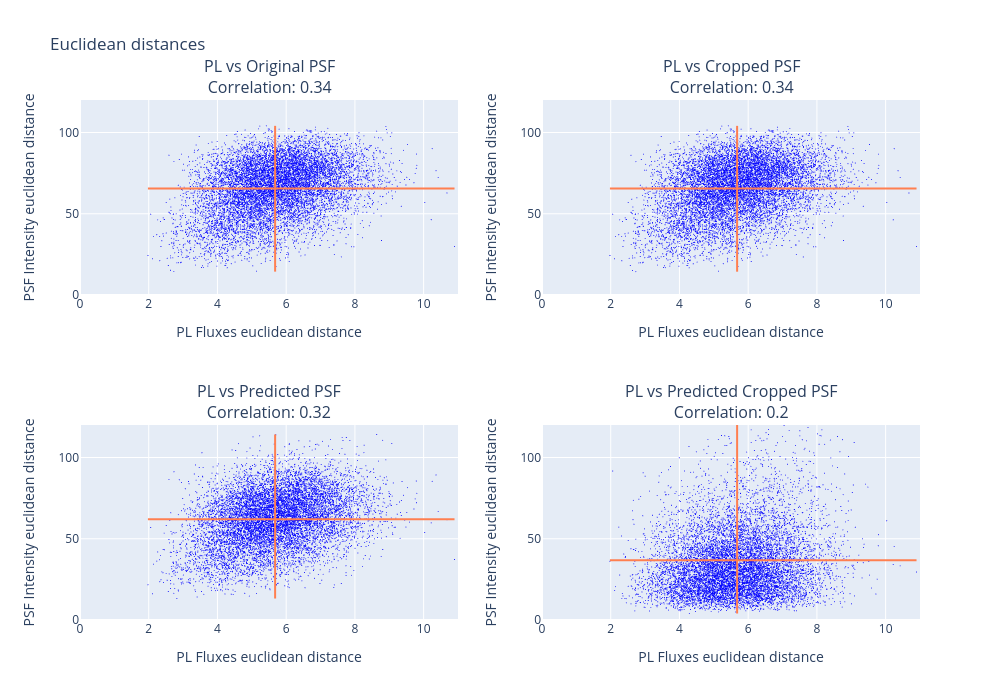
\includegraphics[width=0.7\textwidth]{euclidean_distances.png}}\\
			\subfloat[Euclidean distance ratios]{%
			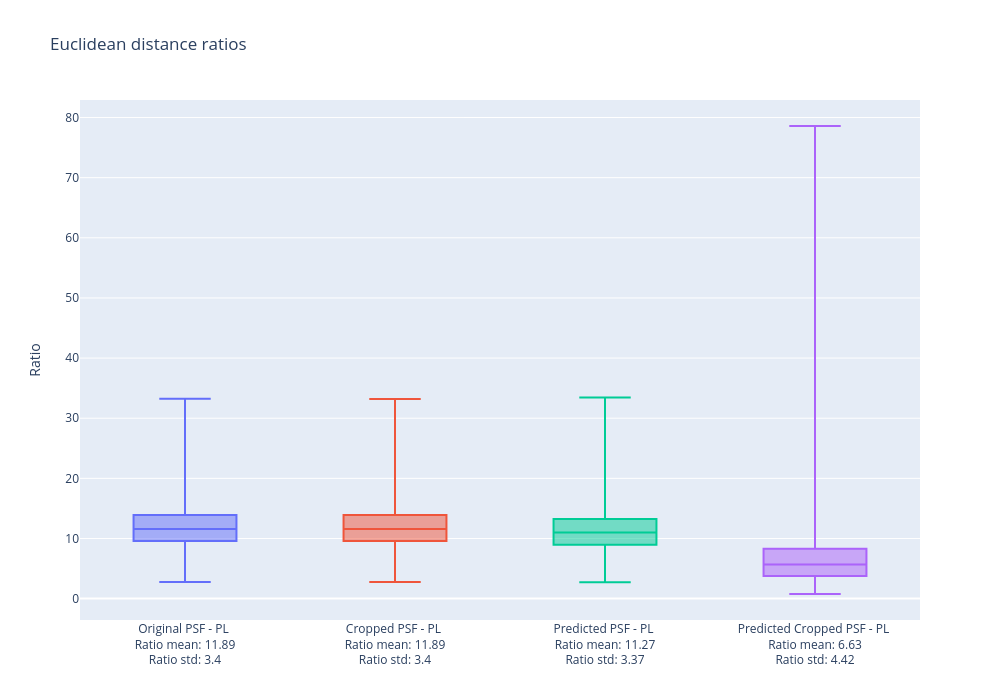
\includegraphics[width=0.7\textwidth]{euclidean_distance_ratios.png}}
			\caption{Euclidean distances ratios between PL and PSF pairs}\hspace{\fill}
		\end{figure*}
		
		After performing an ANOVA test on the euclidean distances from the selected pairs of the 4 datasets obtaining a p-value of 0 and F-statistic of 4789.1531.
		
	\subsubsection{Analysis}
		The correlation is ~0.3 which indicates a slightly positive linear relationship between the PL flux and PSF in all cases except for the cropped predictions which has a 0.2 correlation rate. This makes sense as the model that predicted those PSFs is more overfitted than the model that predicts the original sized PSFs.The clouds are dispersed almost equally from the center of mass which may indicate that a 19 mode PL may not be enough to encode all PSF information. 
